\subsection{AlexNet}
AlexNet is a \acrshort{cnn} developed in 2012 by \textcite{krizhevsky_imagenet_2012}. AlexNet has made a breakthrough in the deep \acrshort{cnn} field and this model has won the ImageNet competition. It is made of 5 convolutional layers and 3 fully-connected layers. We can see the network in Figure \ref{fig:alexnet}. Each convolutional layer has a ReLU activation function and it uses pooling.
%
\begin{figure}
    \centering
    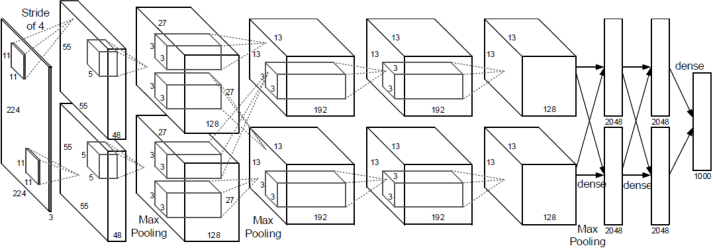
\includegraphics[width=\textwidth]{alexnet.pdf}
    \caption{An illustration of the architecture of AlexNet \cite{krizhevsky_imagenet_2012}}
    \label{fig:alexnet}
\end{figure}
%
\subsection{VGG}
After the success of AlexNet, research has been made to have a network with the same accuracy but lower computational complexity. VGG has been introduced by \textcite{simonyan_very_2015} in 2014, which is a deeper variant of AlexNet. It consists of 5 groups of convolutional layers, where the number of layers depends on the version of VGG. It has won the localization and the second-place tracks in the ImageNet challenge in 2014. An illustration can be found in Figure \ref{fig:vgg}. This depth has been possible by using very small ($3 \times 3$) convolution kernels: it allows a larger receptive field while having fewer parameters and more non-linearities than a larger kernel. However, it has a high memory request. We need 100MB per image to be stored in all \acrshort{fm}s for the forward propagation
%
\begin{figure}
    \centering
    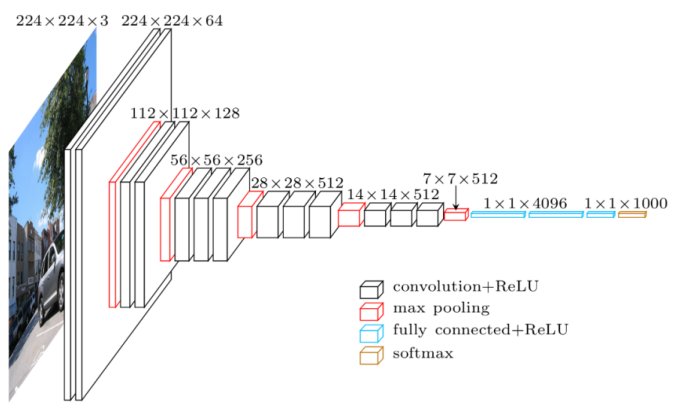
\includegraphics[width=\textwidth]{VGG.pdf}
    \caption{An illustration of the architecture of VGG16 \cite{simonyan_very_2015}}
    \label{fig:vgg}
\end{figure}
%
\subsection{ResNet}
Resnet is a very deep network (between 50 and 1000 convolutional layers) proposed by \textcite{he_deep_2015} with more irregular and complex structures compared to the previous networks. \textcite{he_deep_2015} have shown that an increase of the depth does not mean an improvement in the performance of the network and this is not due to overfitting. It is because the deeper models are harder to optimize than shallower ones (vanishing gradient). But intuitively, the deeper networks should have at least similar or better performance than shallower models. It is explained by the fact that we can map a deeper model into a shallower one by setting the weights to the identity.

Their solution is to add an "identify shortcut connection" that skips one or more layers to mitigate the gradient descent problem and try to set the weights to the identity. We can see the process in figure \ref{fig:resnet}. Weights between the skip connection can be used to learn a residual $F(x)$ to improve the solution. The performance of ResNet allows him to be the 2015 ILSVR winner for both localization and classification.
%
\begin{figure}
    \centering
    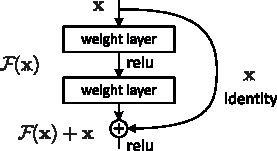
\includegraphics[width=0.8\textwidth]{resnet.pdf}
    \caption{ResNet building block \cite{he_deep_2015}}
    \label{fig:resnet}
\end{figure}
%
\subsection{MobileNetV2} \label{subs:mbv2}
The drive of the previous networks for accuracy has come for high computational and storage costs which are beyond de capabilities of many mobiles and embedded applications, according to \textcite{cheng_recent_2018}. For the \acrshort{cnn} training phase, it is not a problem thanks to the high performance and large disk and memory storage capacities of the \acrshort{gpu} and \acrshort{cpu} clouds. However, for the inference stage, it is difficult to deploy such networks on mobile devices such as \acrshort{fpga} because of their constraint resources:
%
\begin{itemize}
    \item The enormous computational complexity of \acrshort{cnn}s makes it difficult to deploy on real-time applications and it consumes battery power.
    \item The large number of parameters of \acrshort{cnn}s consumes considerable storage and run-time memory.
\end{itemize}

\textcite{sandler_mobilenetv2_2019} have proposed a network tailored for such constrained environments. To do so, we must first reduce the size and number of operations. They have achieved it using \acrshort{dsc}, introduced in section \ref{subs:dsc}, and a new kind of layer: inverted residual with a linear bottleneck (observed in figure \ref{fig:invreslinbot}). It is first composed of a $1 \times 1$ convolution to expand the number of the input \acrshort{fm} channels and then followed by a \acrshort{dsc}. The intermediate increase in the number of channels is supposed to counterbalance the loss of information that occurred by the ReLU. They have also added a skip connection to build a network of great depth, and the last convolution has a linear activation function.
%
\begin{figure}
    \centering
    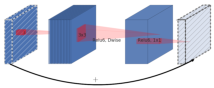
\includegraphics[width=\textwidth]{mbnv2.pdf}
    \caption{inverted residual with linear bottleneck \cite{sandler_mobilenetv2_2019}}
    \label{fig:invreslinbot}
\end{figure}
